\documentclass[tikz, border=3.14mm]{standalone}
\usepackage{pgfplots}
\pgfplotsset{compat=1.18}

\begin{document}
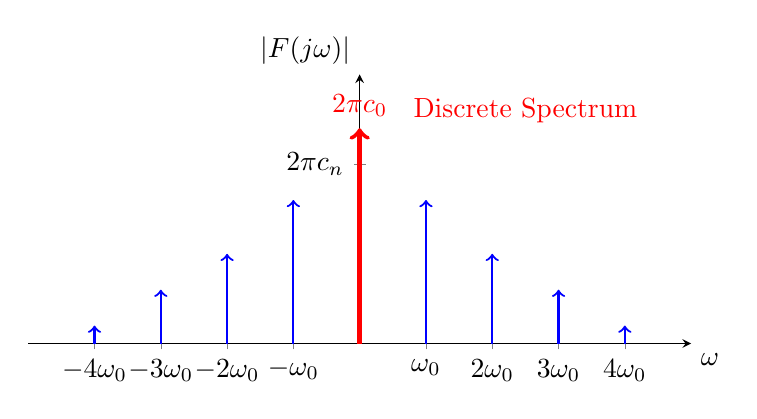
\begin{tikzpicture}
    \begin{axis}[
        axis lines = middle,
        xlabel = {$\omega$},
        ylabel = {$|F(j\omega)|$},
        xmin = -5, xmax = 5,
        ymin = 0, ymax = 1.5,
        xtick = {-4, -3, -2, -1, 1, 2, 3, 4},
        xticklabels = {$-4\omega_0$, $-3\omega_0$, $-2\omega_0$, $-\omega_0$, $\omega_0$, $2\omega_0$, $3\omega_0$, $4\omega_0$},
        ytick = {1},
        yticklabels = {$2\pi c_n$},
        width = 10cm, height = 5cm,
        grid = none,
        every axis x label/.style={at={(current axis.right of origin)},anchor=north west},
        every axis y label/.style={at={(current axis.above origin)},anchor=south east},
    ]
        % Discrete impulses at n*omega_0
        \draw[ultra thick, red, ->] (axis cs:0,0) -- (axis cs:0,1.2) node[anchor=south] {$2\pi c_0$};
        \draw[thick, blue, ->] (axis cs:1,0) -- (axis cs:1,0.8);
        \draw[thick, blue, ->] (axis cs:-1,0) -- (axis cs:-1,0.8);
        \draw[thick, blue, ->] (axis cs:2,0) -- (axis cs:2,0.5);
        \draw[thick, blue, ->] (axis cs:-2,0) -- (axis cs:-2,0.5);
        \draw[thick, blue, ->] (axis cs:3,0) -- (axis cs:3,0.3);
        \draw[thick, blue, ->] (axis cs:-3,0) -- (axis cs:-3,0.3);
        \draw[thick, blue, ->] (axis cs:4,0) -- (axis cs:4,0.1);
        \draw[thick, blue, ->] (axis cs:-4,0) -- (axis cs:-4,0.1);
        
        \node[red] at (axis cs: 2.5, 1.3) {Discrete Spectrum};

    \end{axis}
\end{tikzpicture}
\end{document}
